\section{Figures}

\begin{figure}[htp]
  \centering
  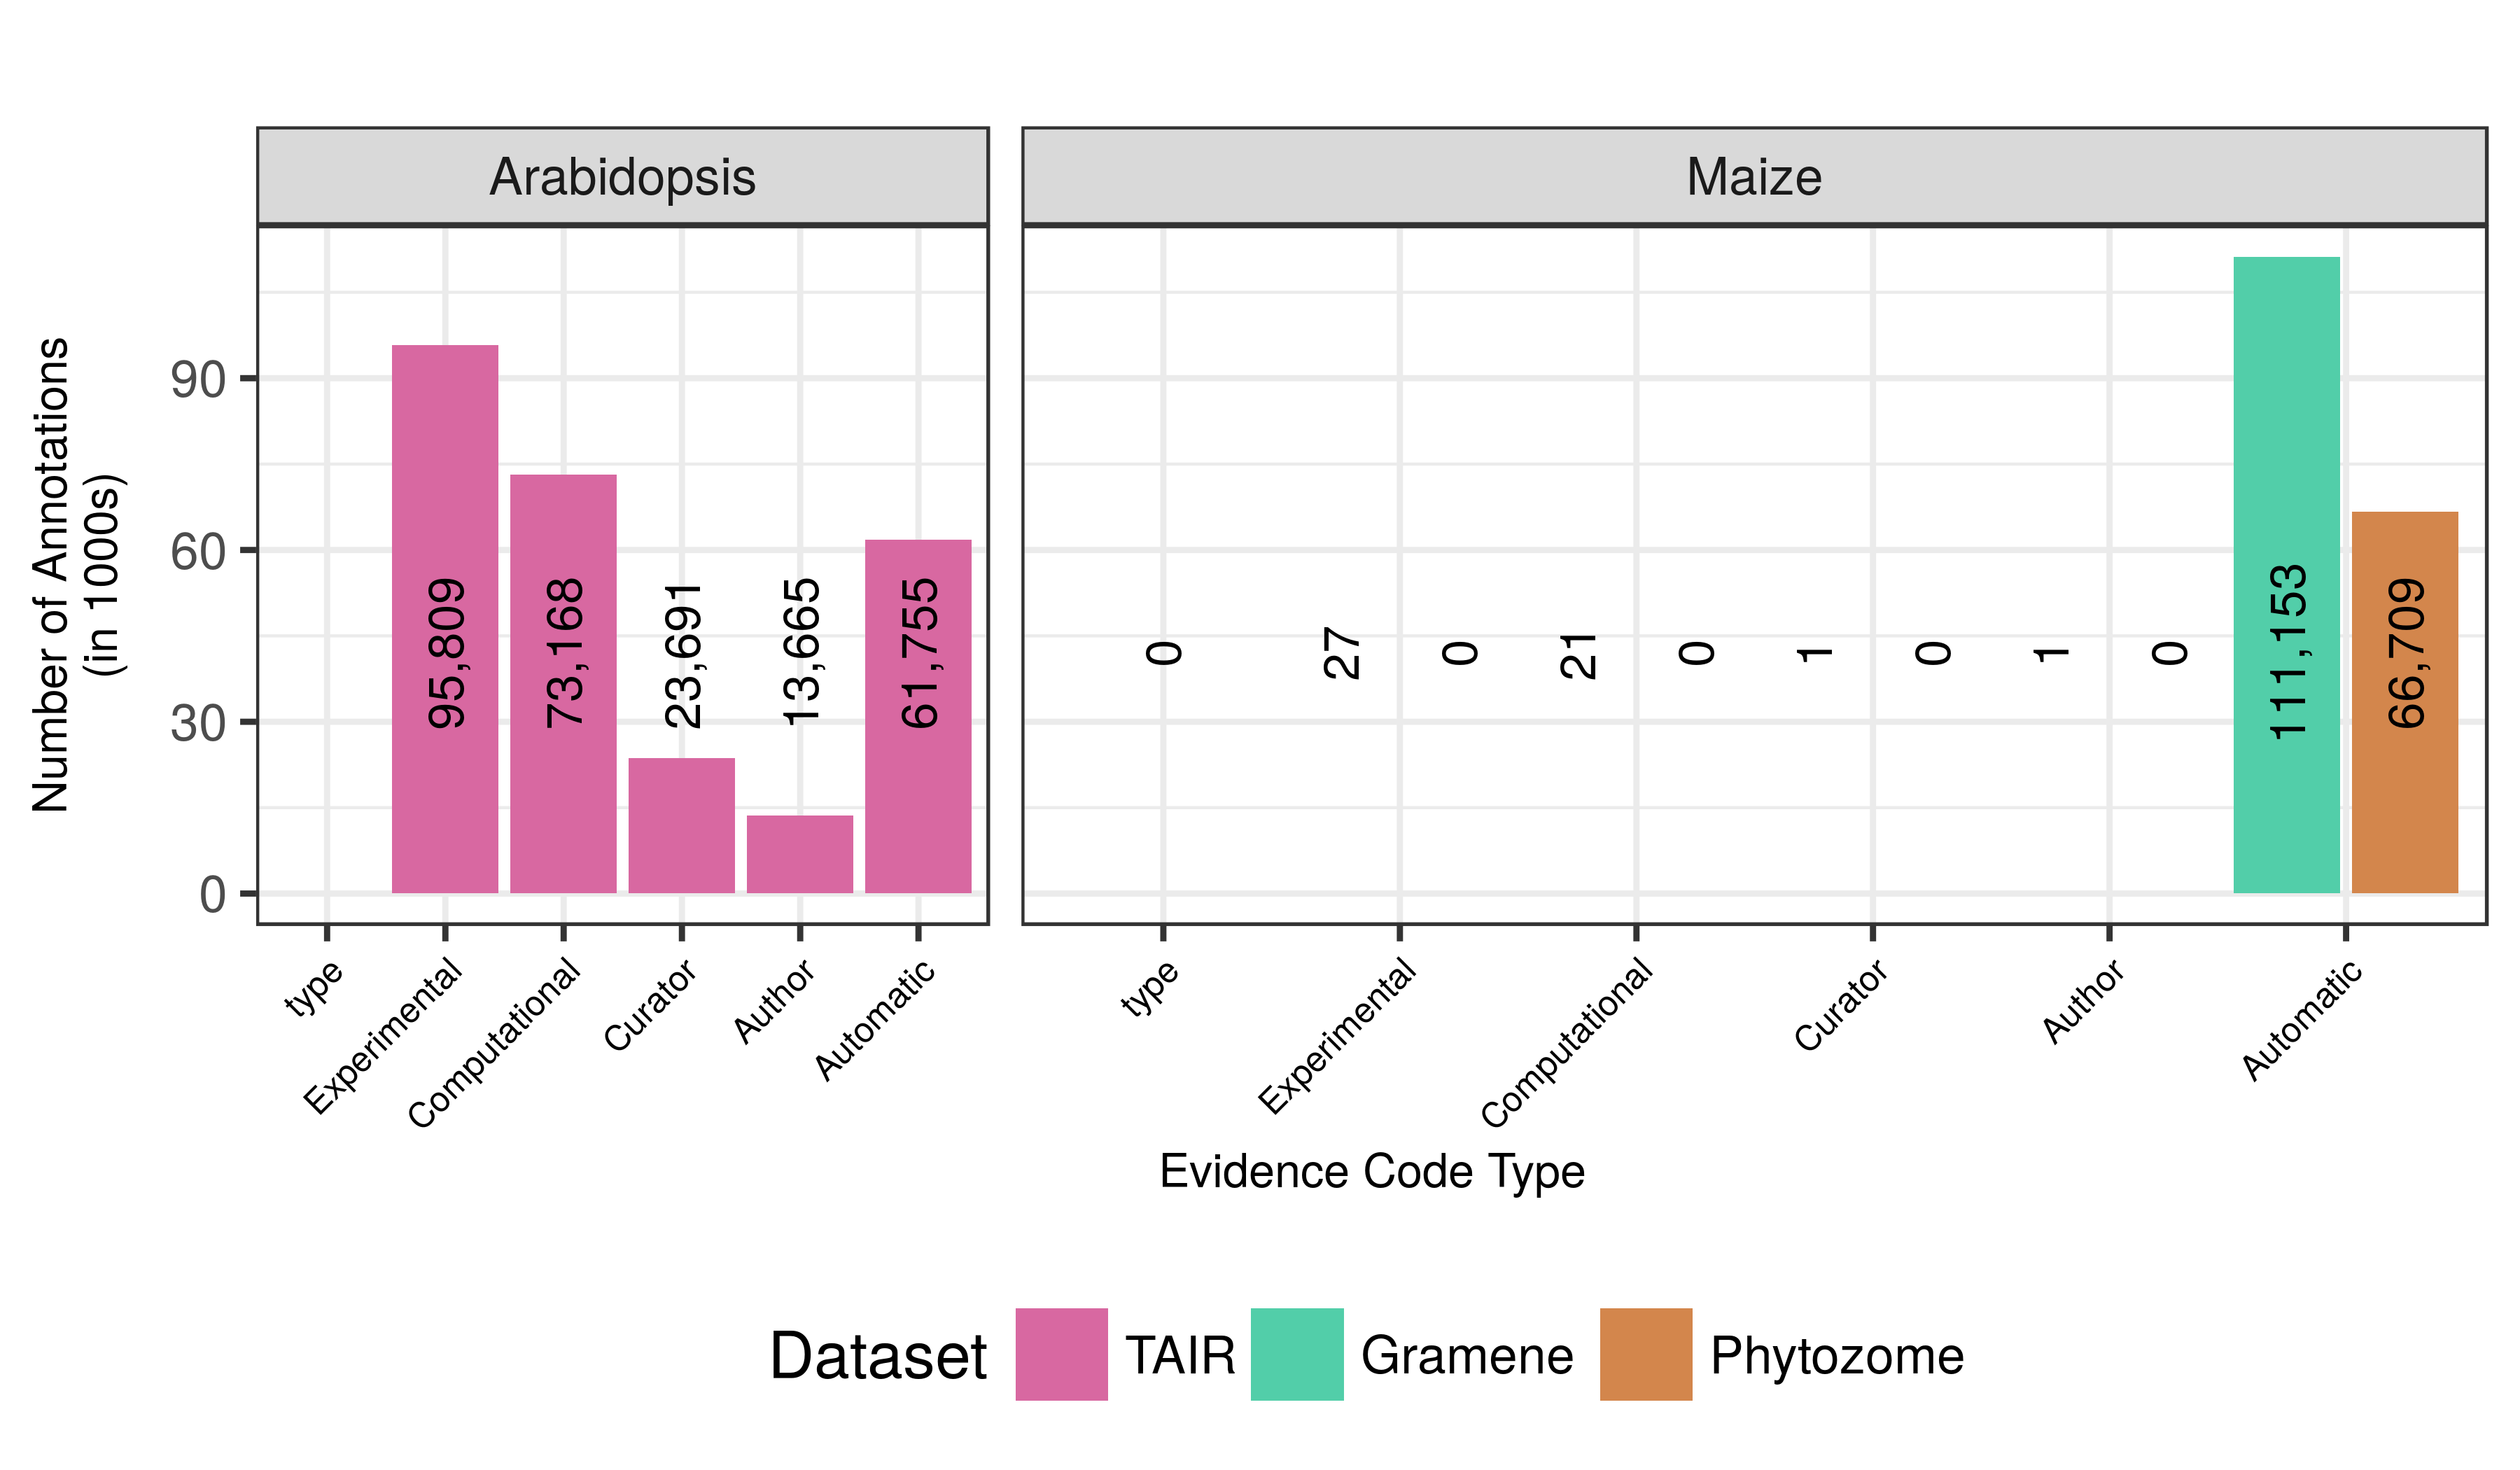
\includegraphics[width=\textwidth]{figures/figure1/all_annots.png}
  \caption{\textbf{Numbers of annotations by EC category.}}
  \raggedright
  Arabidopsis (TAIR10) shown in magenta, maize in green and orange for Gramene and Phytozome, respectively. Annotation counts on the y-axis are shown in thousands. Each bar in the histogram is labeled with the actual count to show where counts are so small that no bar is visible.
  \label{fig:num_annots}
\end{figure}

%\newpage

\begin{figure}[htp]
  \centering
  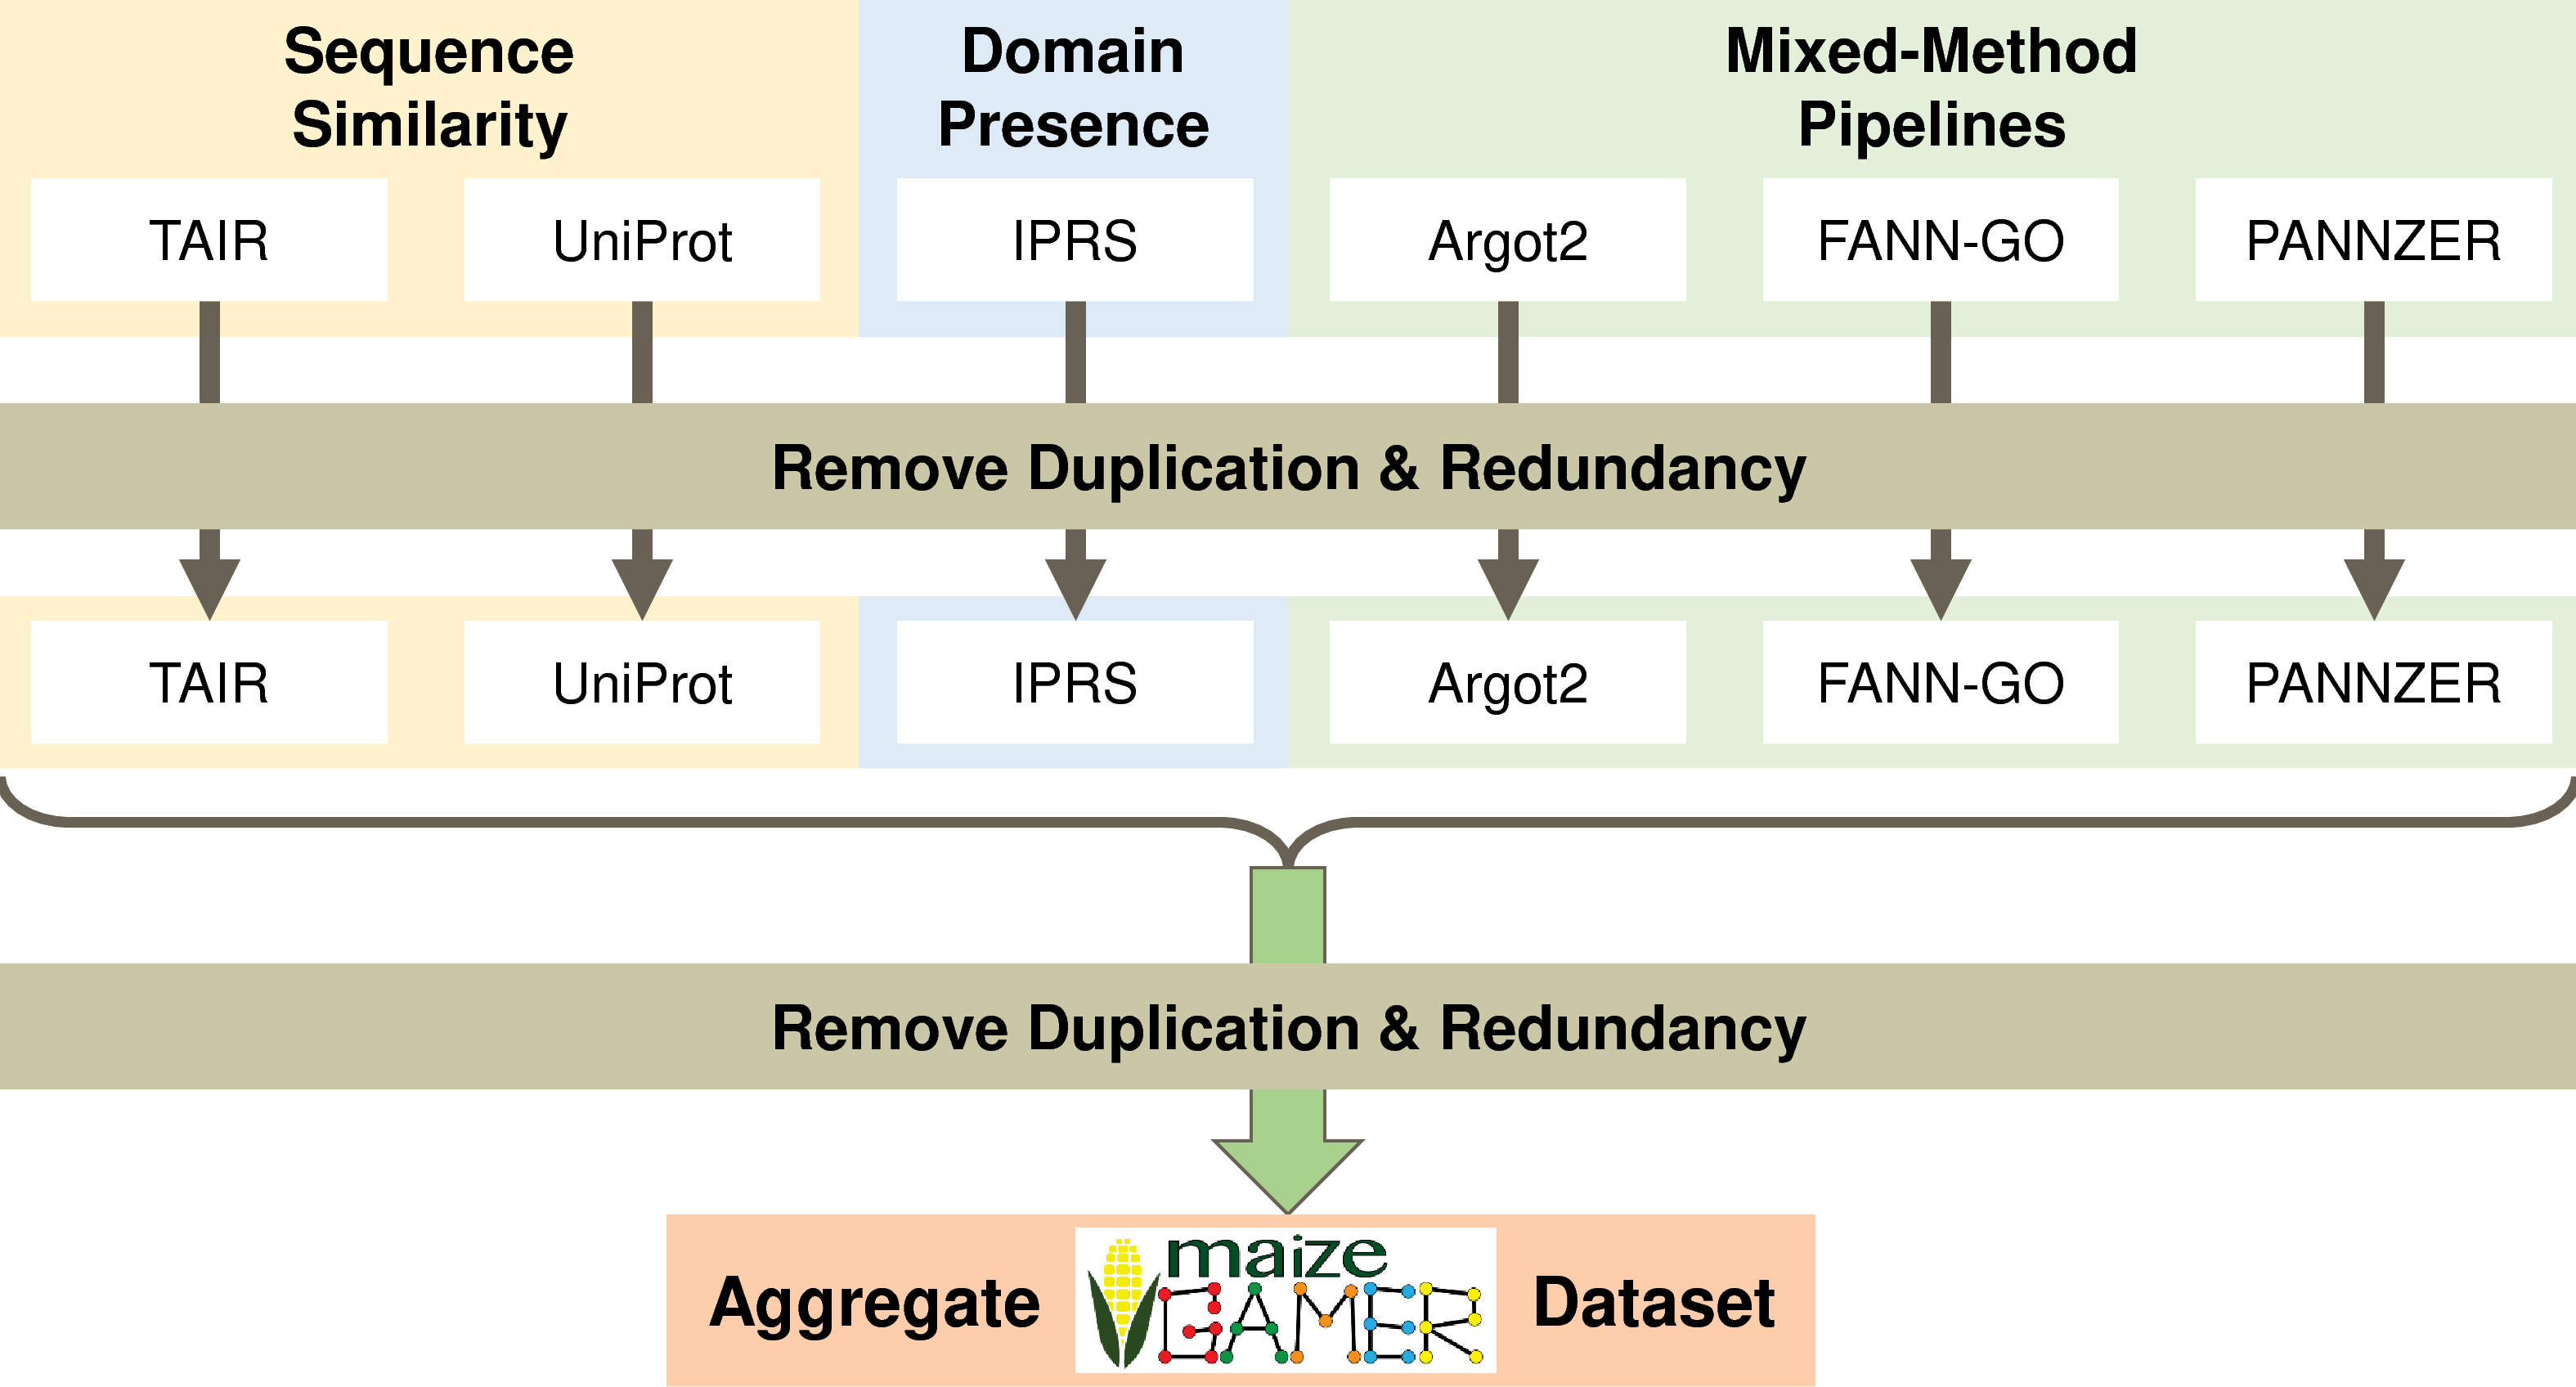
\includegraphics[width=0.7\textwidth]{figures/figure2/methods-1.png}
  \caption{\textbf{Overview of steps to produce the maize-GAMER datasets.}}
  \raggedright
  Three types of methods are used: sequence similarity (yellow), domain presence, (blue) and CAFA mixed-method pipelines (green). Within sequence similarity, two input datasets were subjected to reciprocal-best-hit against maize: TAIR10 (Arabidopsis) and UniProt (the ten most well-annotated plant species).  For domain presence, InterPro signatures were applied to maize using InterProScan (IPRS). From the CAFA mixed-method pipelines, Argot2, FANN-GO, and PANNZER were applied to maize. For each individual output, duplications and redundancies were removed, then the datasets were combined. A second round of duplication and redundancy removal was carried out to produce the aggregate maize-GAMER dataset.
  \label{fig:methods}
\end{figure}

\begin{figure}[htp]
  \centering
  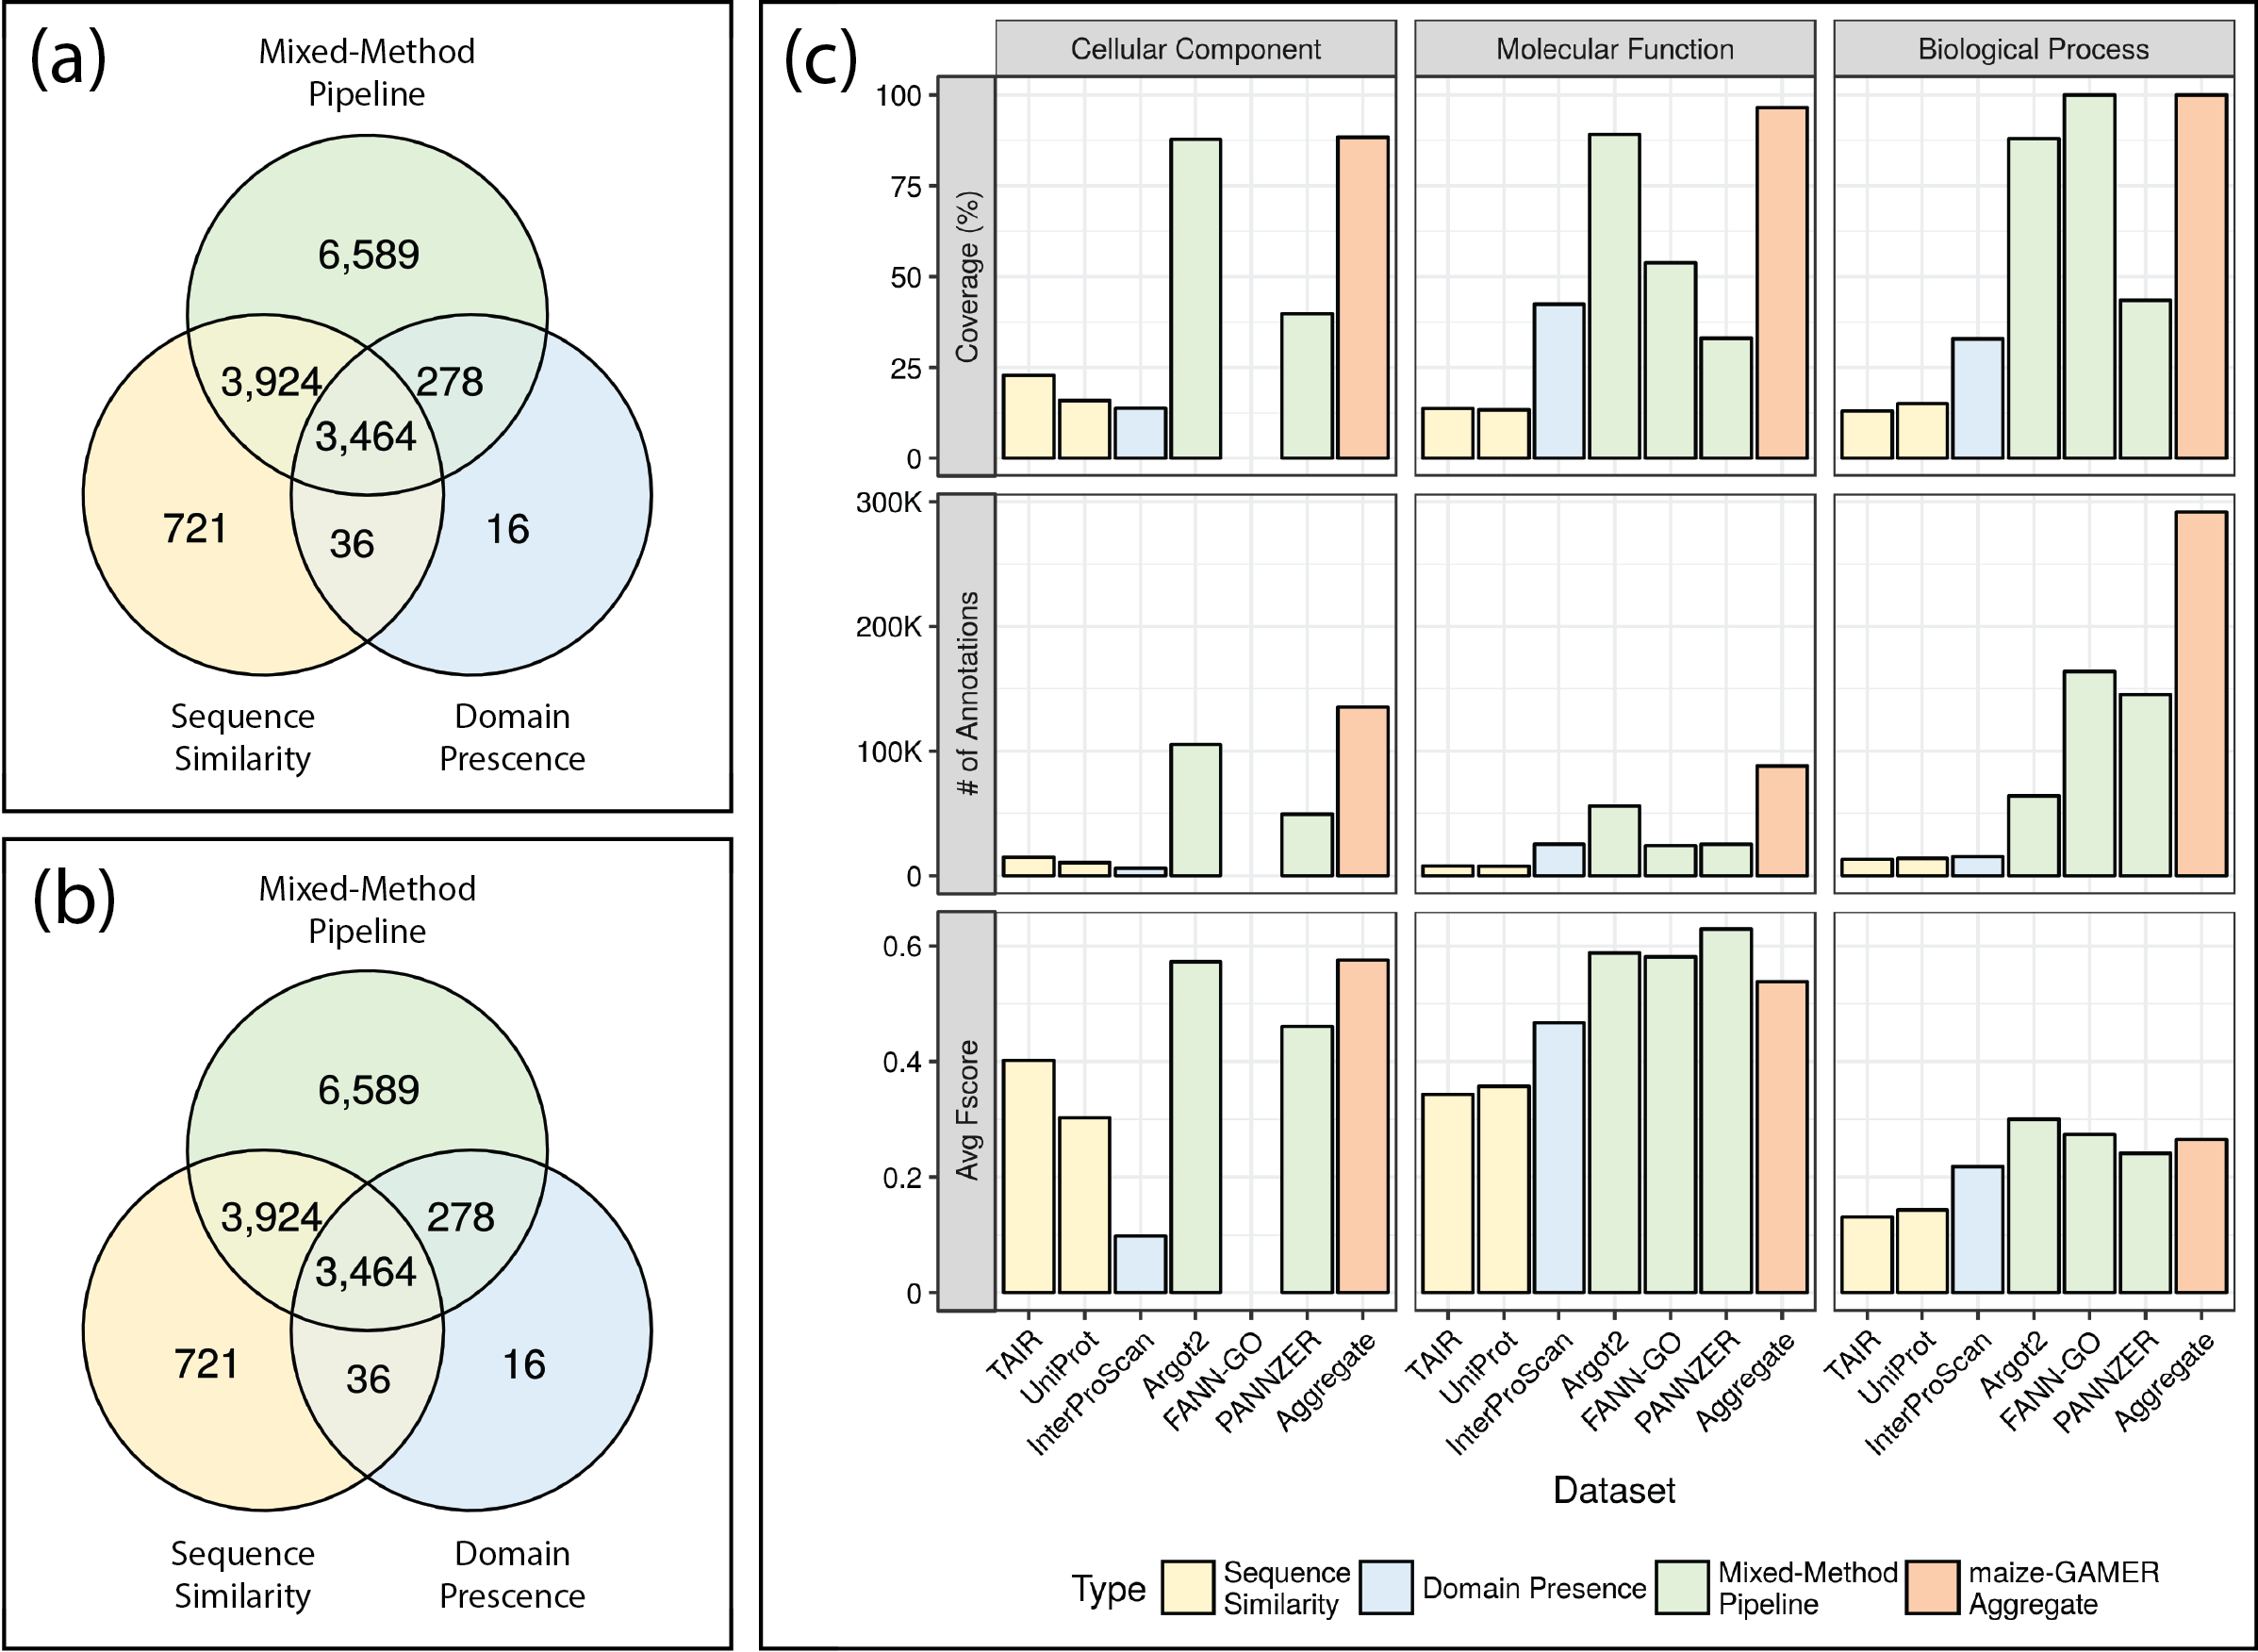
\includegraphics[width=\textwidth]{figures/figure3/figure3.png}
  \caption{\textbf{GO assignment metrics for each method type.}}
  \raggedright
  Sequence similarity in yellow, domain presence in blue, and mixed-method pipeline in green. (a) Number of genes with at least one GO term annotated.  (b) Number of GO terms with at least one gene annotated. (c) Percent coverage, number of annotations, and average $hF_1$ score for each annotation dataset across the three GO graphs (i.e., Cellular Component, Molecular Function, and Biological Process). Color codes as described in a and b, with the aggregate dataset shown in orange.
  \label{fig:maize_gam_eval}
\end{figure}

\begin{figure}[htp]
  \centering
  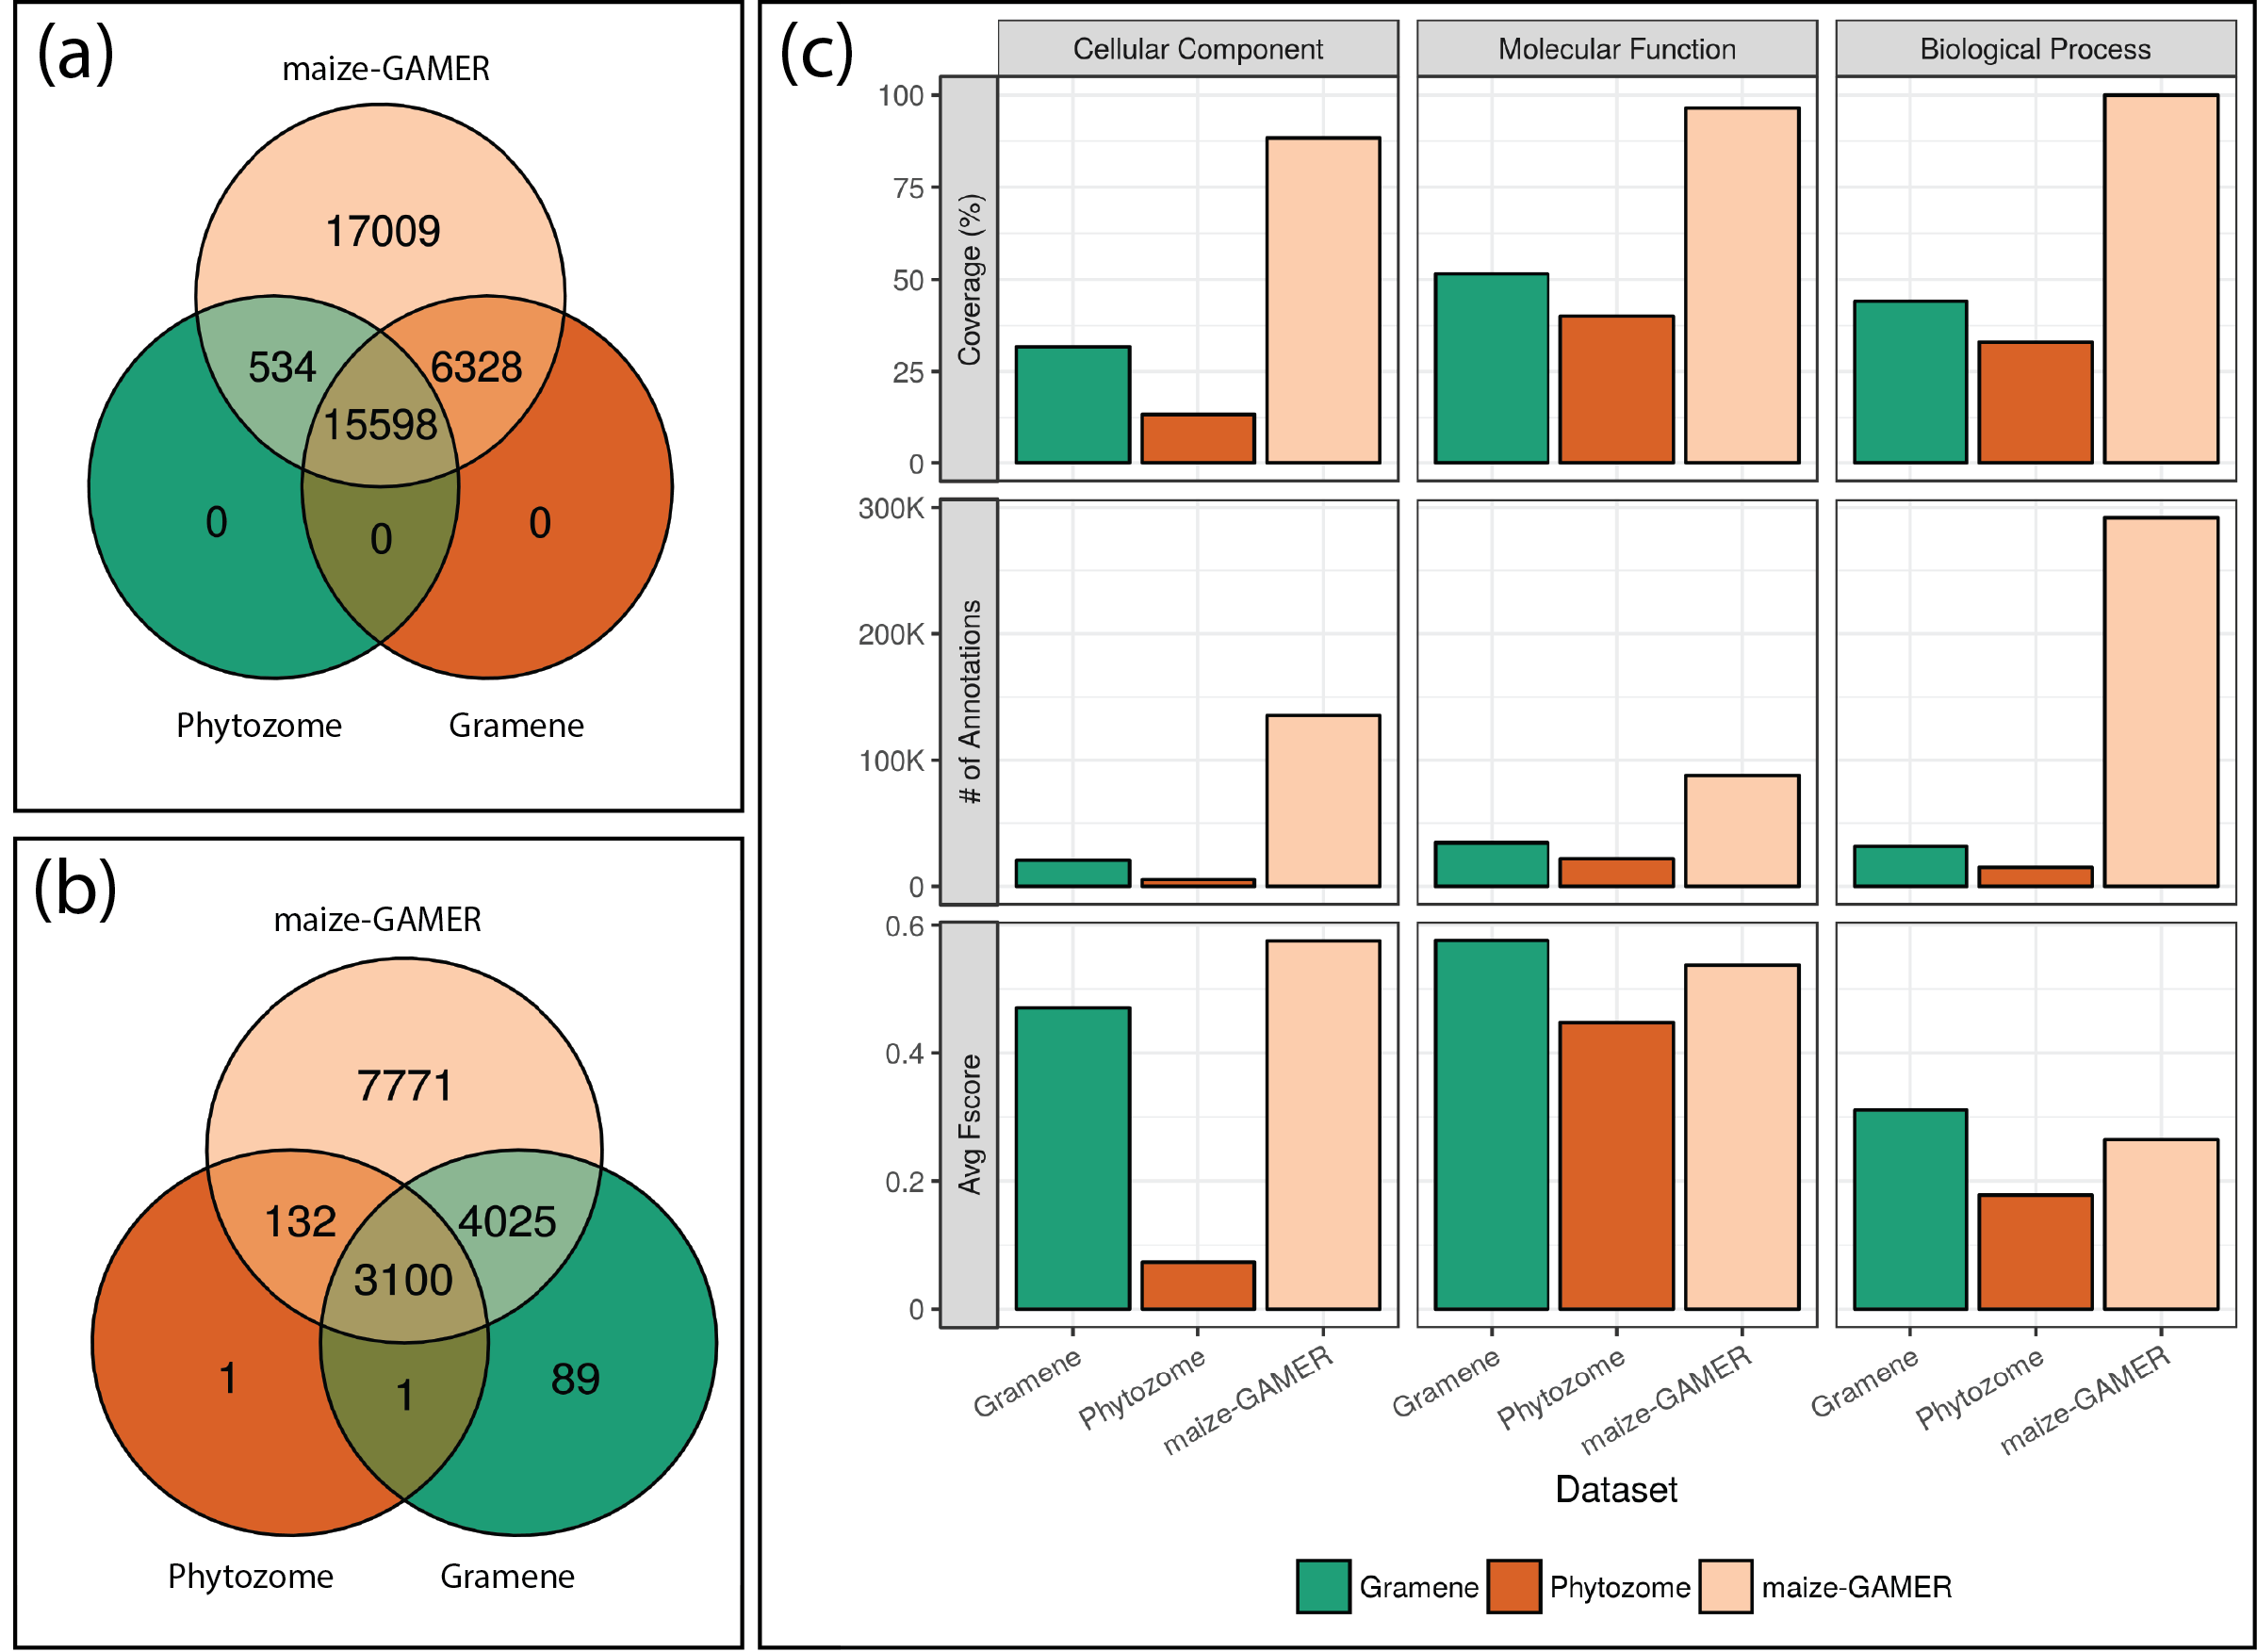
\includegraphics[width=\textwidth]{figures/figure4/figure4.png}
  \caption{\textbf{GO assignment metrics for Gramene, Phytozome, and maize-GAMER.}}
  \raggedright
  Gramene in green, Phytozome in rust, and maize-GAMER in tan. (a) Number of genes with at least one GO term annotated.  (b) Number of GO terms with at least one gene annotated. (c) Percent coverage, number of annotations, and $hF_1$ score for each annotation dataset across the three GO graphs (i.e., Cellular Component, Molecular Function, and Biological Process).
  \label{fig:maize_dataset_eval}
\end{figure}


\begin{figure}[htp]
  \centering
  \begin{subfigure}[t]{\textwidth}
        \centering
        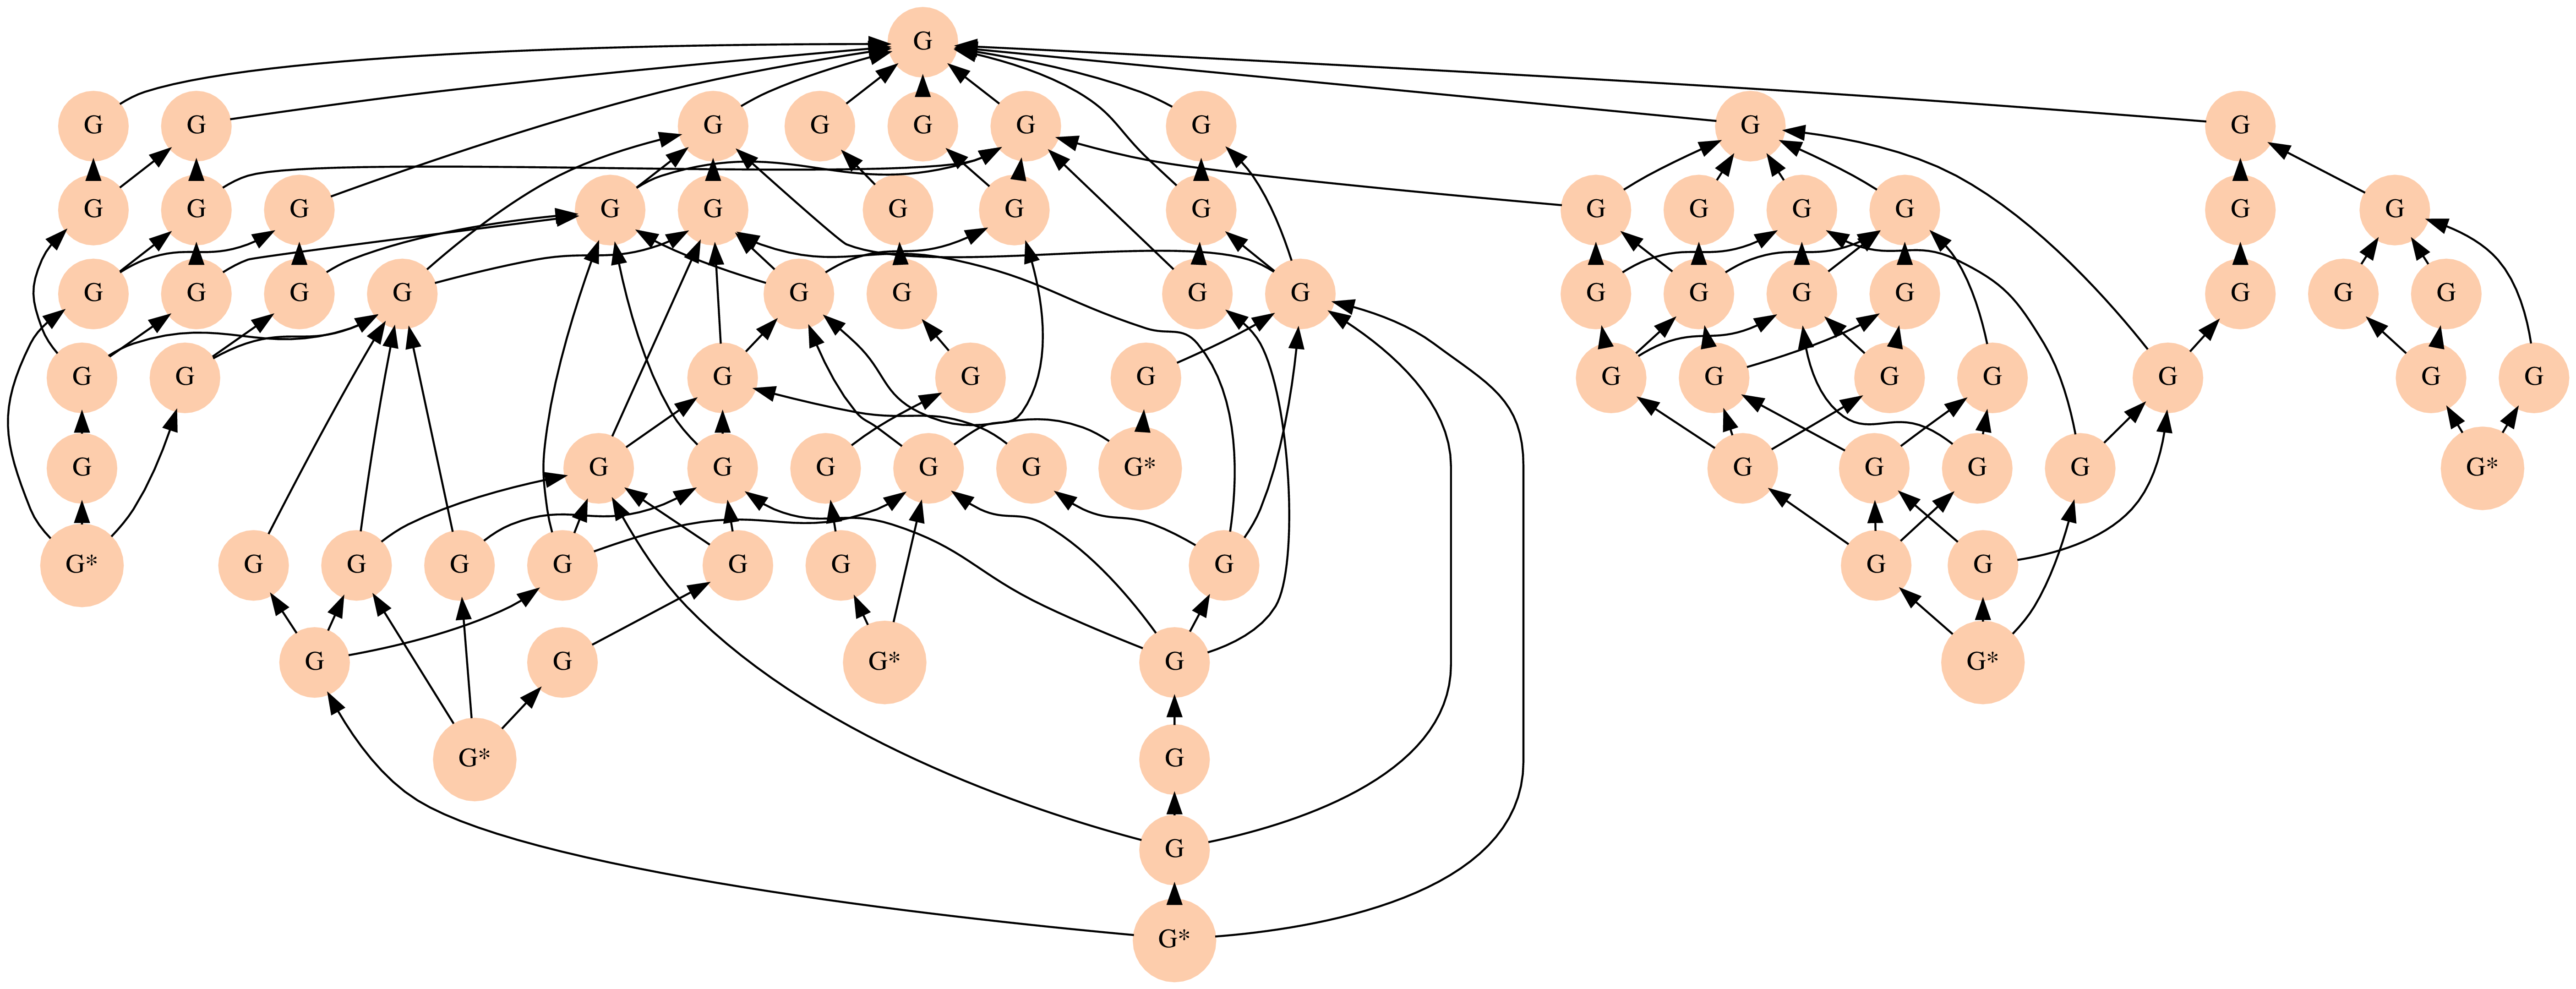
\includegraphics[width=0.65\textwidth]{figures/figure5/phytozome_data.png}
        \caption{Phytozome Annotations}
        \label{fig:phytozome_na1}
  \end{subfigure}%
  \\
  \begin{subfigure}[t]{\textwidth}
        \centering
        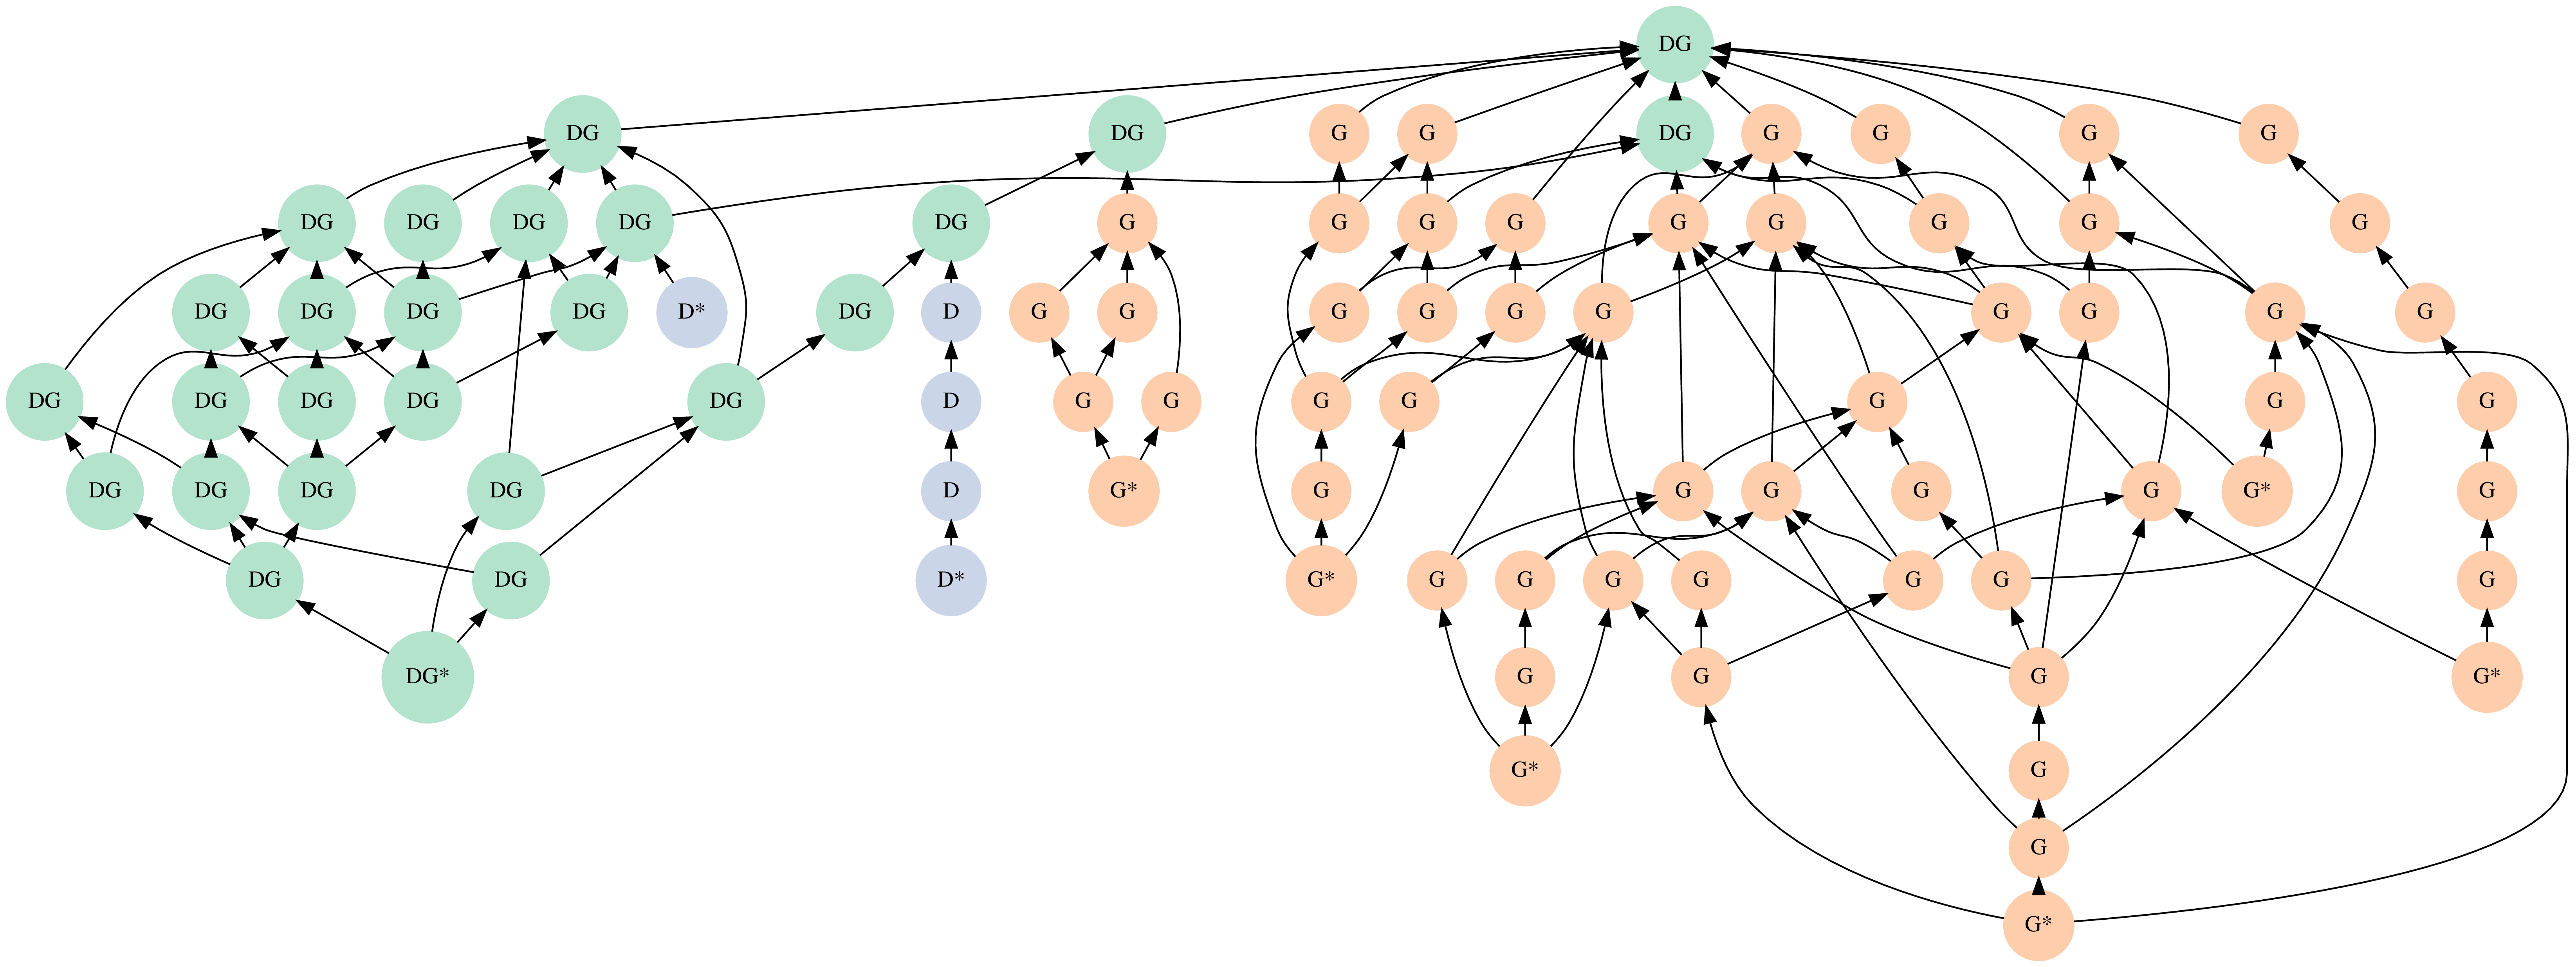
\includegraphics[width=0.76\textwidth]{figures/figure5/gramene_data.png}
        \caption{Gramene Annotations}
        \label{fig:gramene_na1}
  \end{subfigure}%
  \\
  \begin{subfigure}[t]{\textwidth}
        \centering
        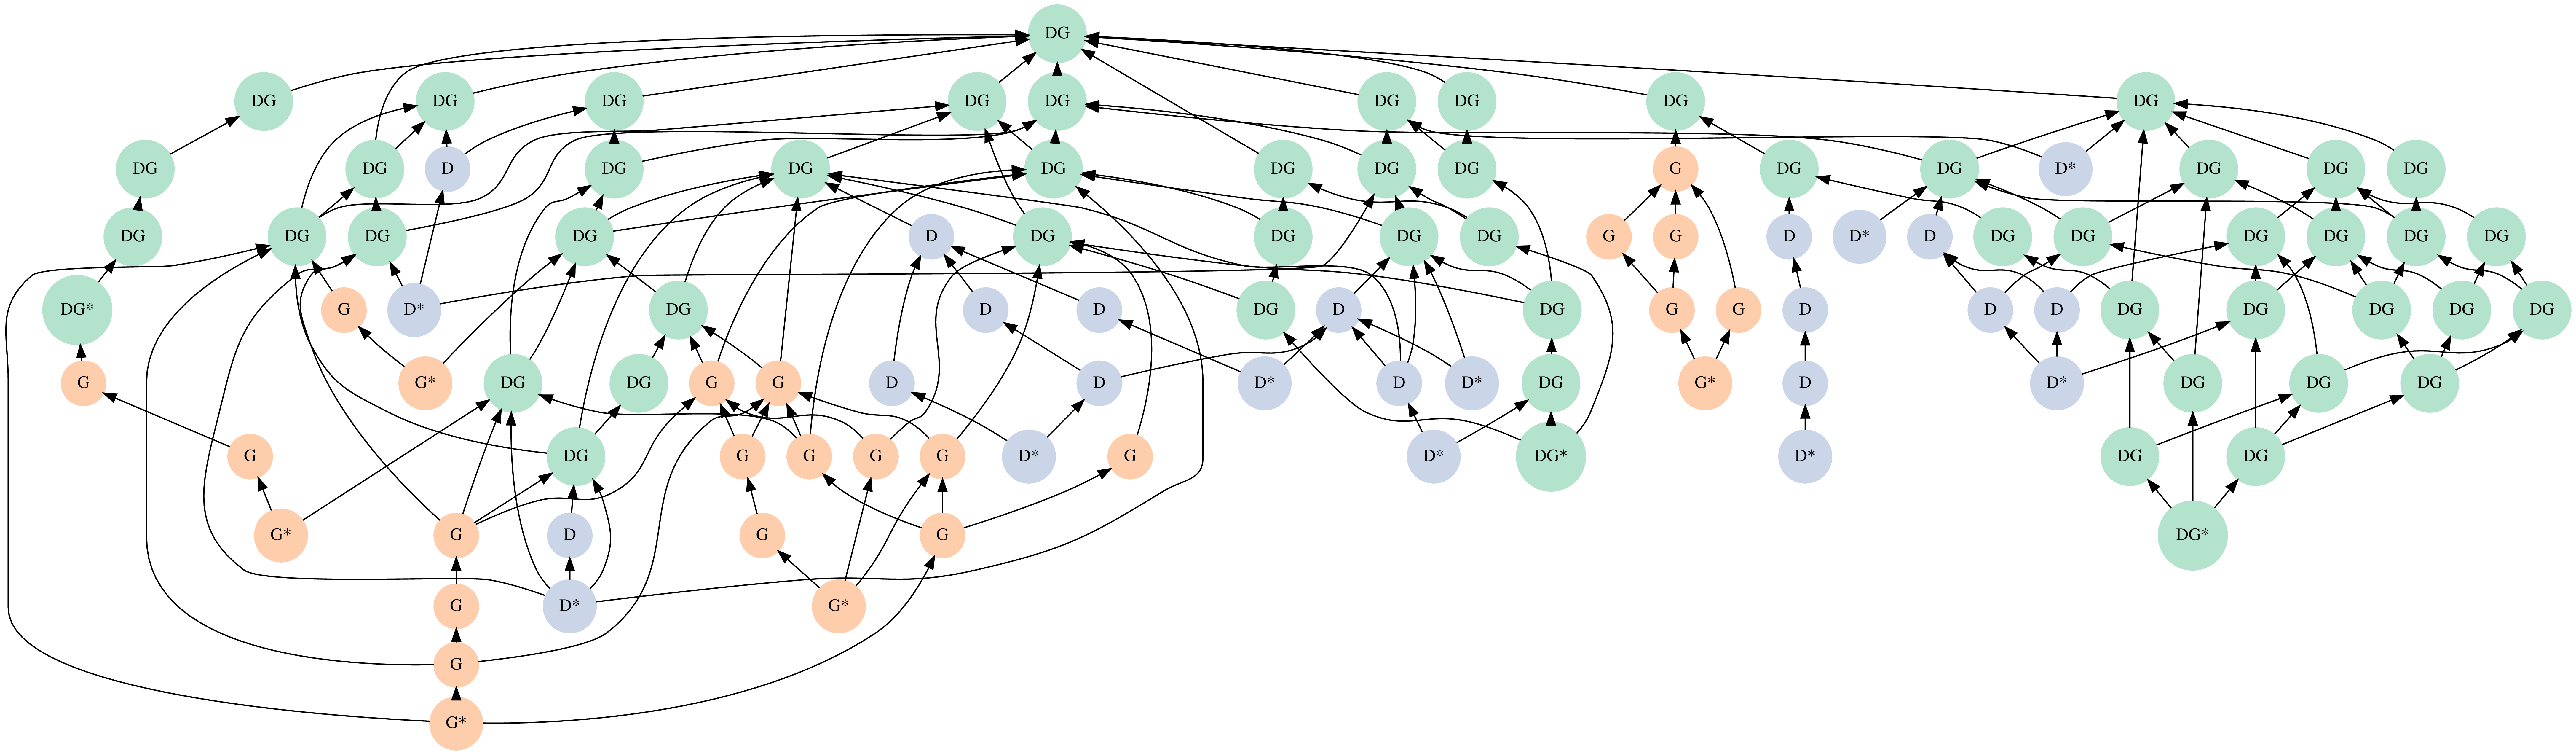
\includegraphics[width=\textwidth]{figures/figure5/gamer_data.png}
        \caption{maize-GAMER Annotations}
        \label{fig:gamer_na1}
  \end{subfigure}%
%  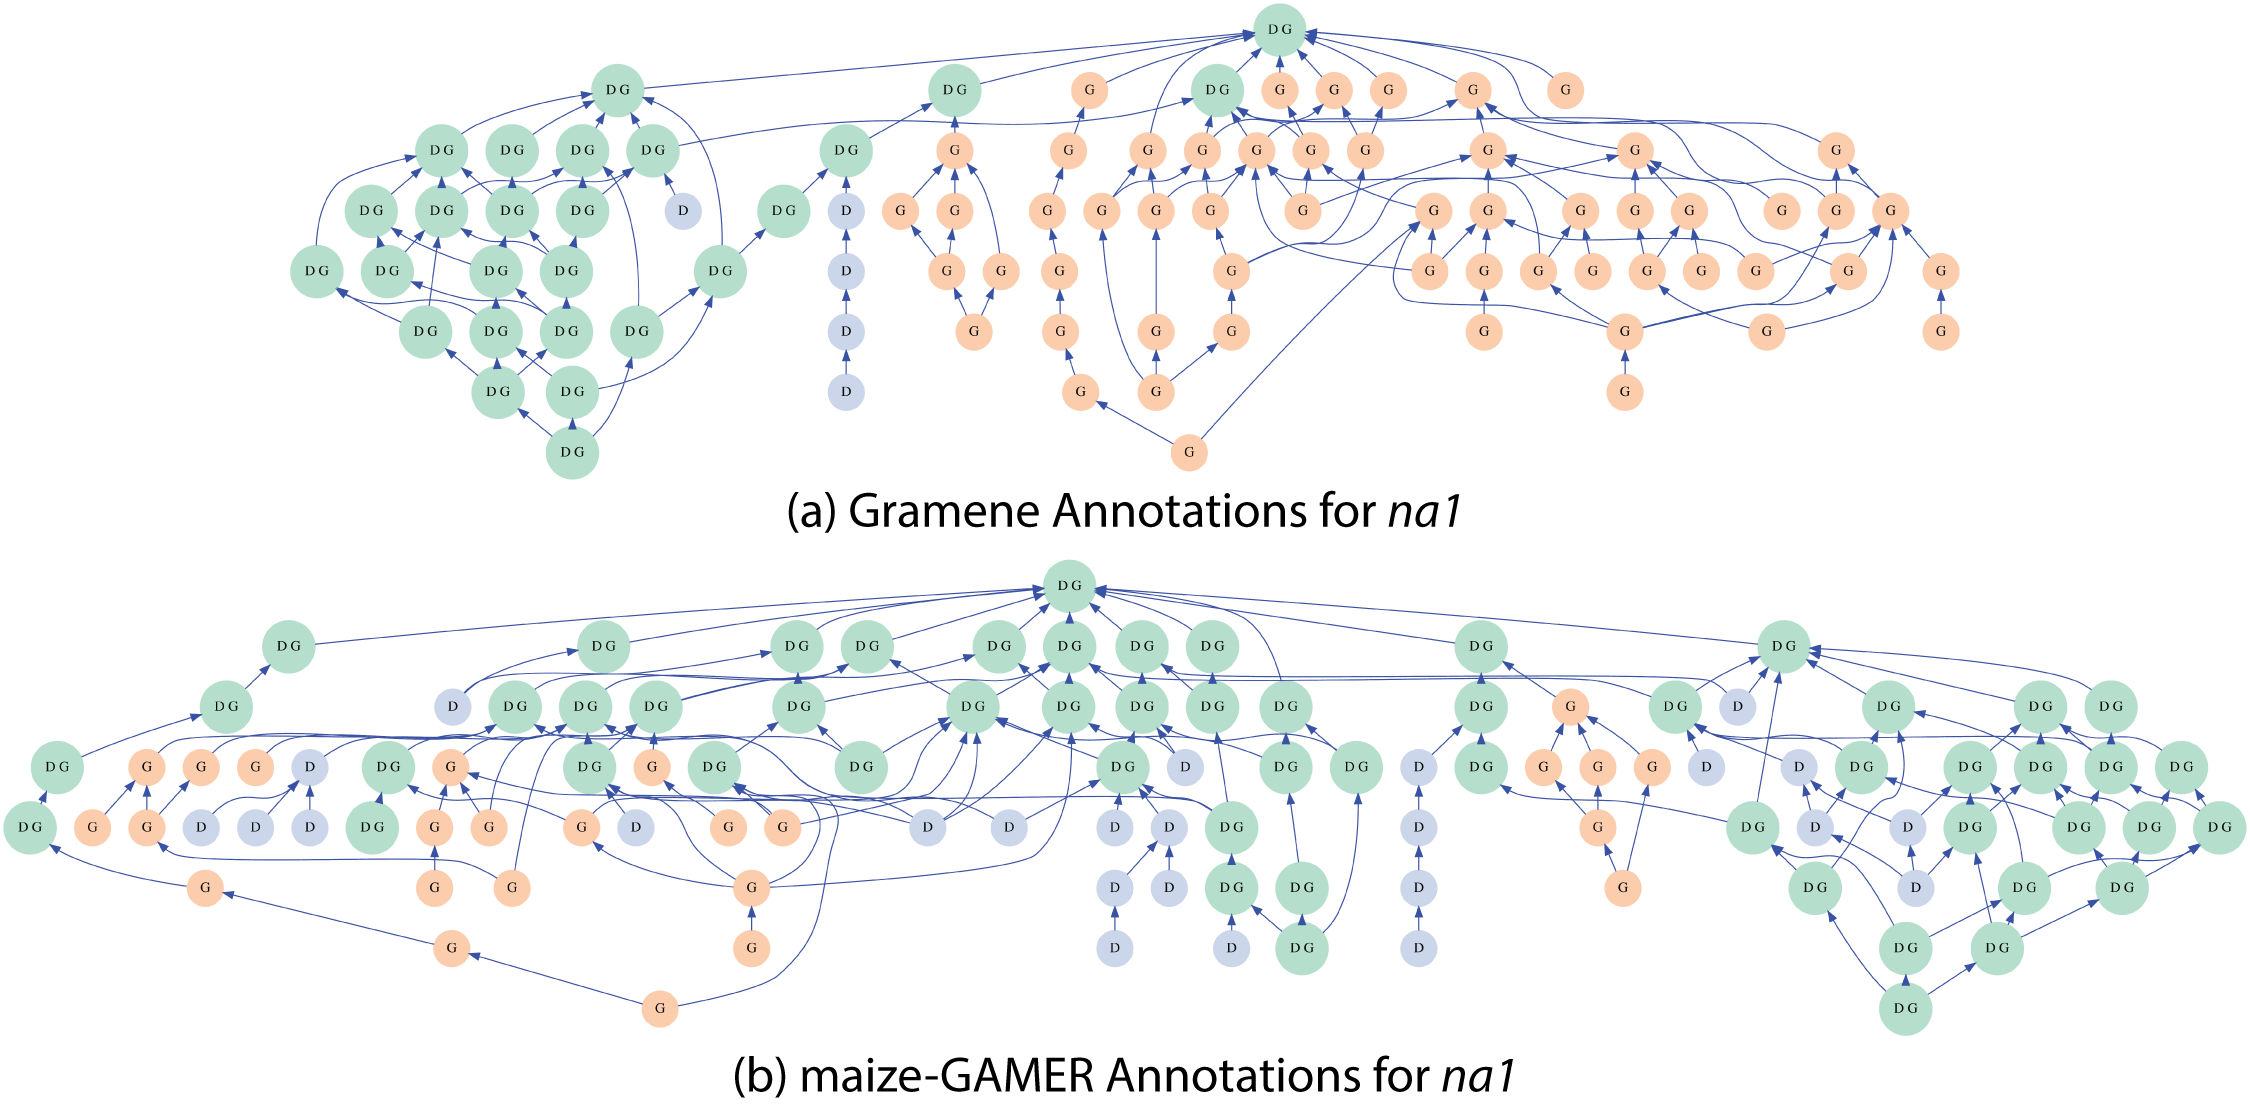
\includegraphics[width=\textwidth]{figures/figure5/figure5.png}
  \caption{\textbf{Biological Process GO graph for maize \textit{na1}.}}
  \raggedright
  Leaf terms are toward the bottom, root terms are toward the top.  Terms covered only by the gold standard are shown in orange (labeled G), those in the dataset but absent from the gold standard are shown in blue (labeled D), and those that appear in both are shown in green (labeled DG). Leaf terms in each subgraph have an * next to them. Phytozome graph is shown at the top \ref{fig:phytozome_na1} Gramene graph is shown in the middle \ref{fig:gramene_na1}, and maize-GAMER aggregate graph is shown at the bottom \ref{fig:gamer_na1}.
  \label{fig:na1_diagram}
\end{figure}
